

\begin{algorithm}
    \caption{Fluorescence segmentation}\label{alg:global-thresholding}
    \begin{algorithmic}
    \item 1. Normalize image
    \item 2. Apply global \textit{threshold\_mean} to receive initial mask.
    \item 3. Zero out pixels outside the mask
    \item 4. Apply local thresholding.  
    \item 5. Apply \textit{fill\_holes} transformation.
    \item 6. Morphological opening from opencv and Gaussian blur.
    \item 7. Run \textit{findContours} from opencv in order to obtain separate regions and filter out too small regions.
    \end{algorithmic}
\end{algorithm}    

Segmentation steps are also illustrated in Figure \begin{figure}[H]
    \centering
    \setkeys{Gin}{width=\linewidth}
    \centering
        \begin{tabularx}{\textwidth}{YYYYYYY}
            \textbf{1} &
            \textbf{2} &
            \textbf{3} &
            \textbf{4} &
            \textbf{5} &
            \textbf{6} &
            \textbf{7} \\
            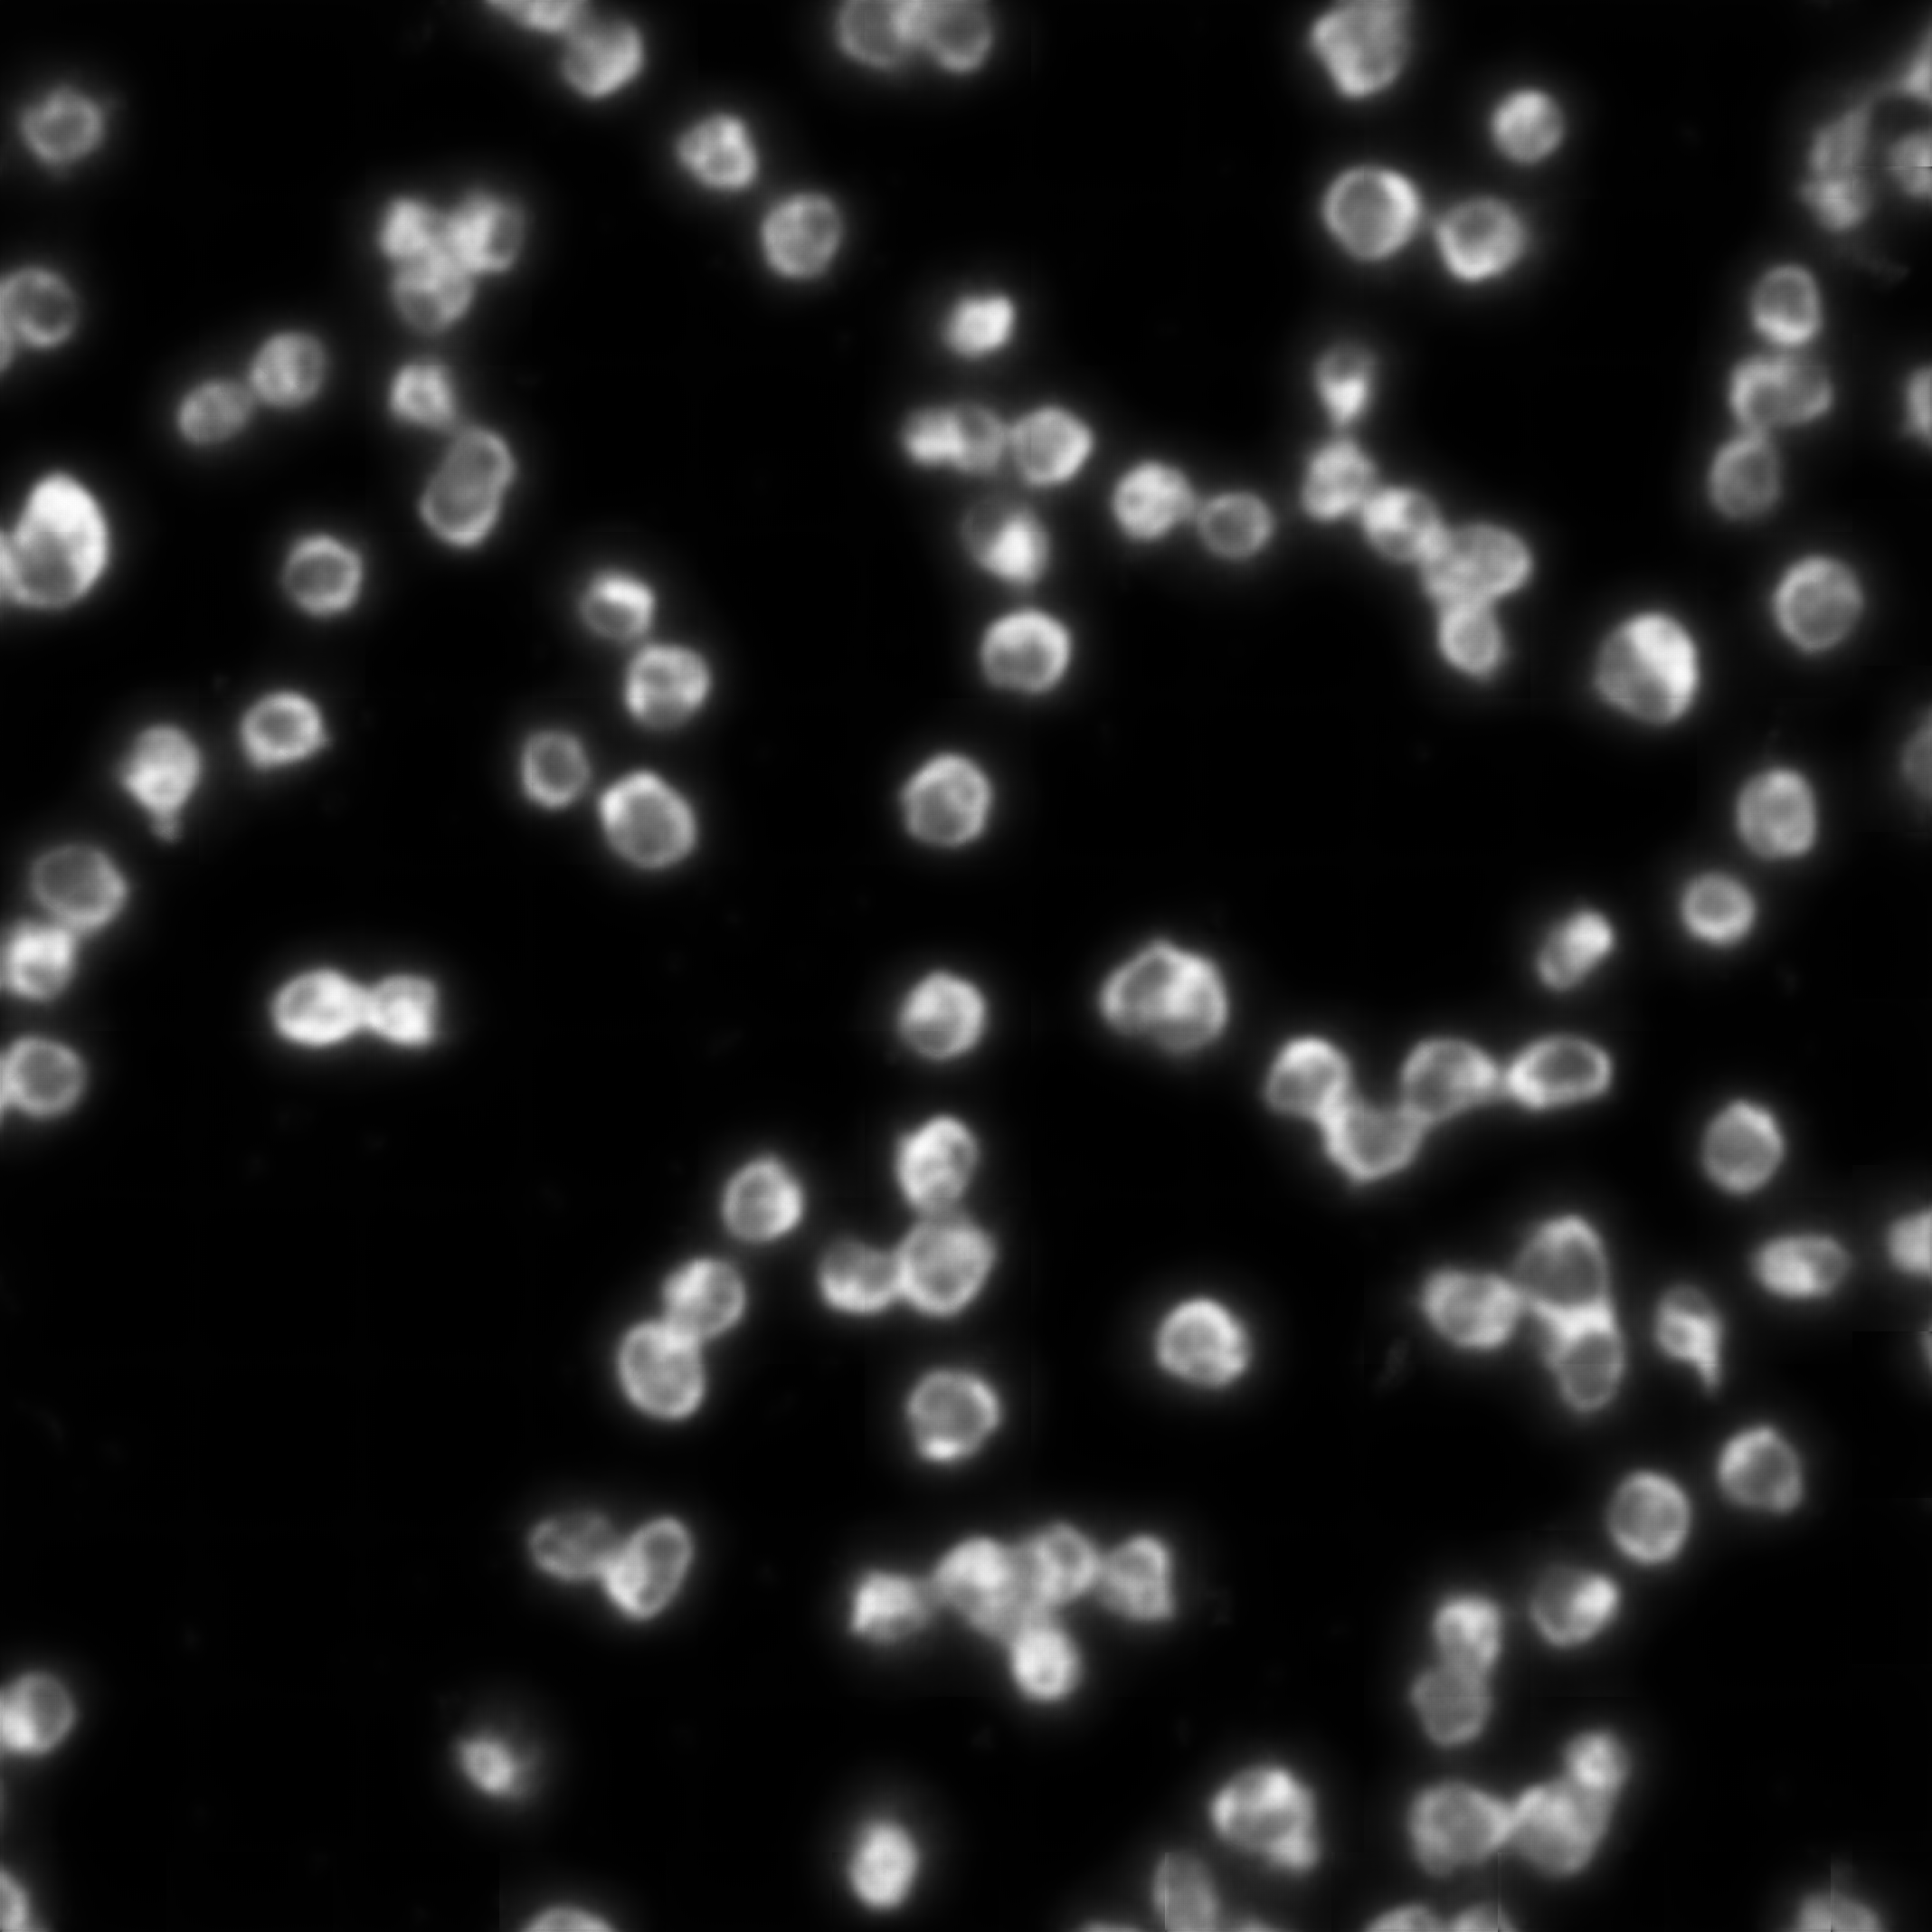
\includegraphics{bilder/ER/segmentation/pp_1.png} & 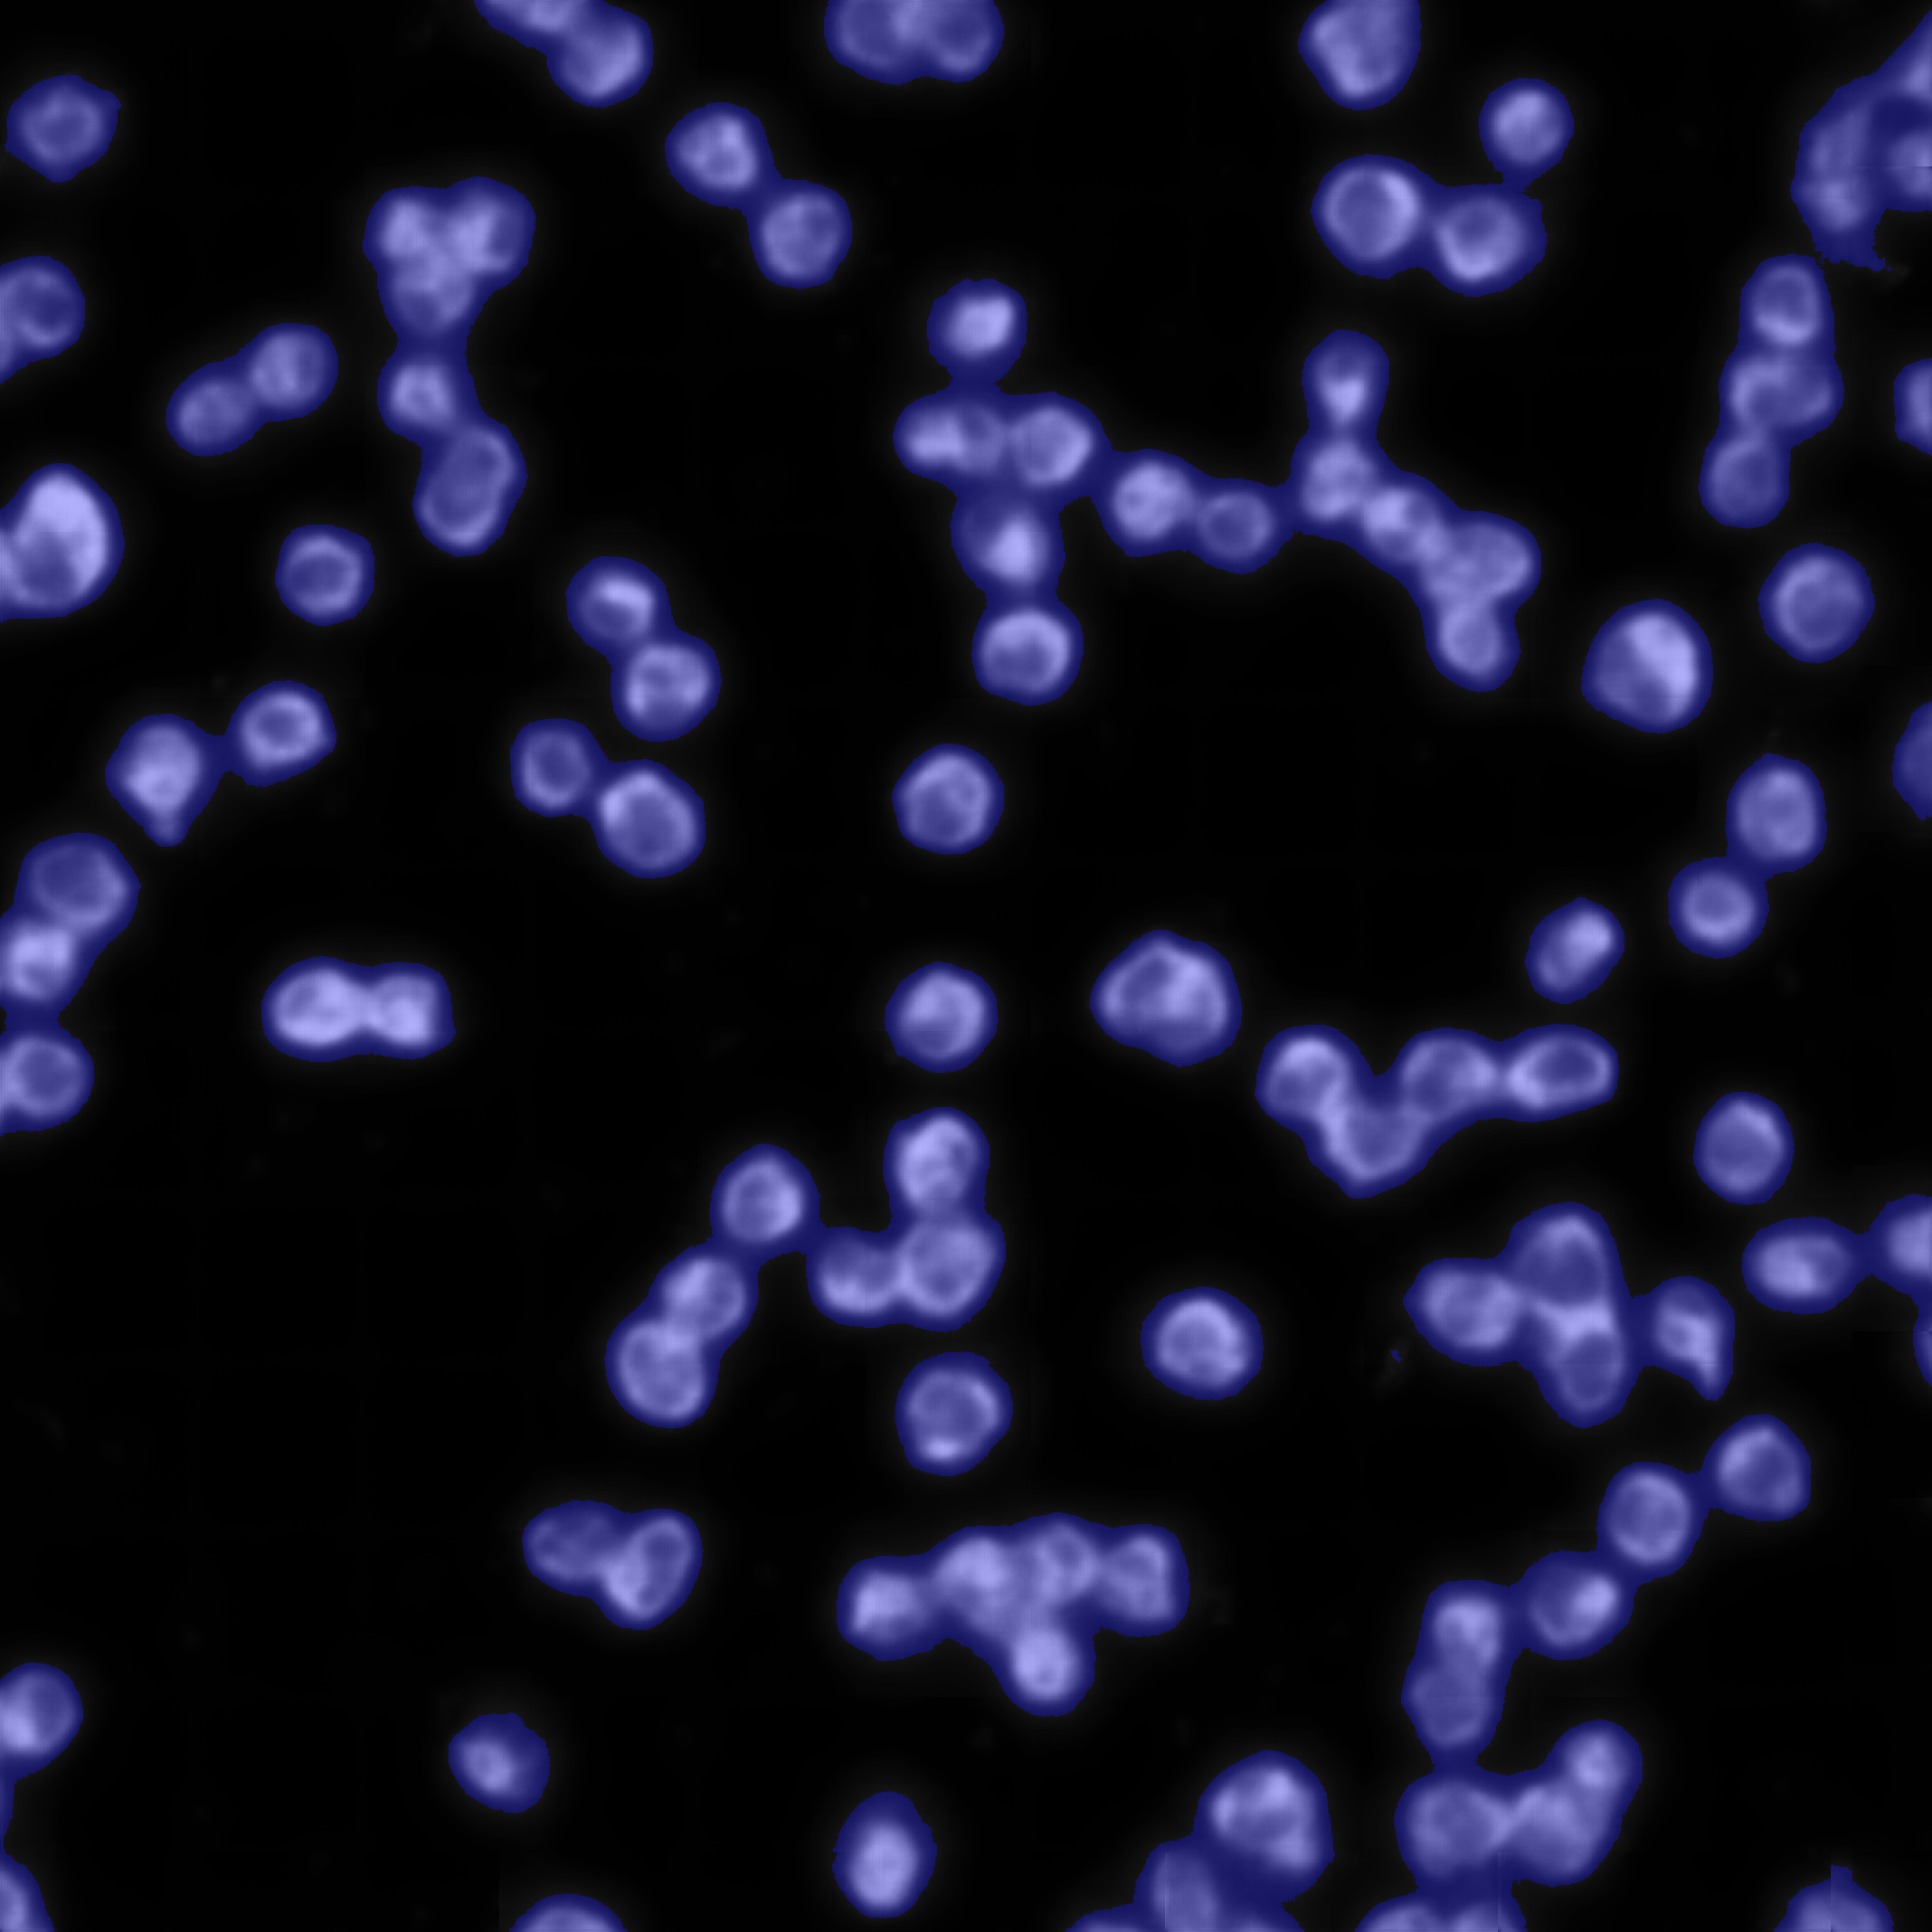
\includegraphics{bilder/ER/segmentation/pp_2.png} &
            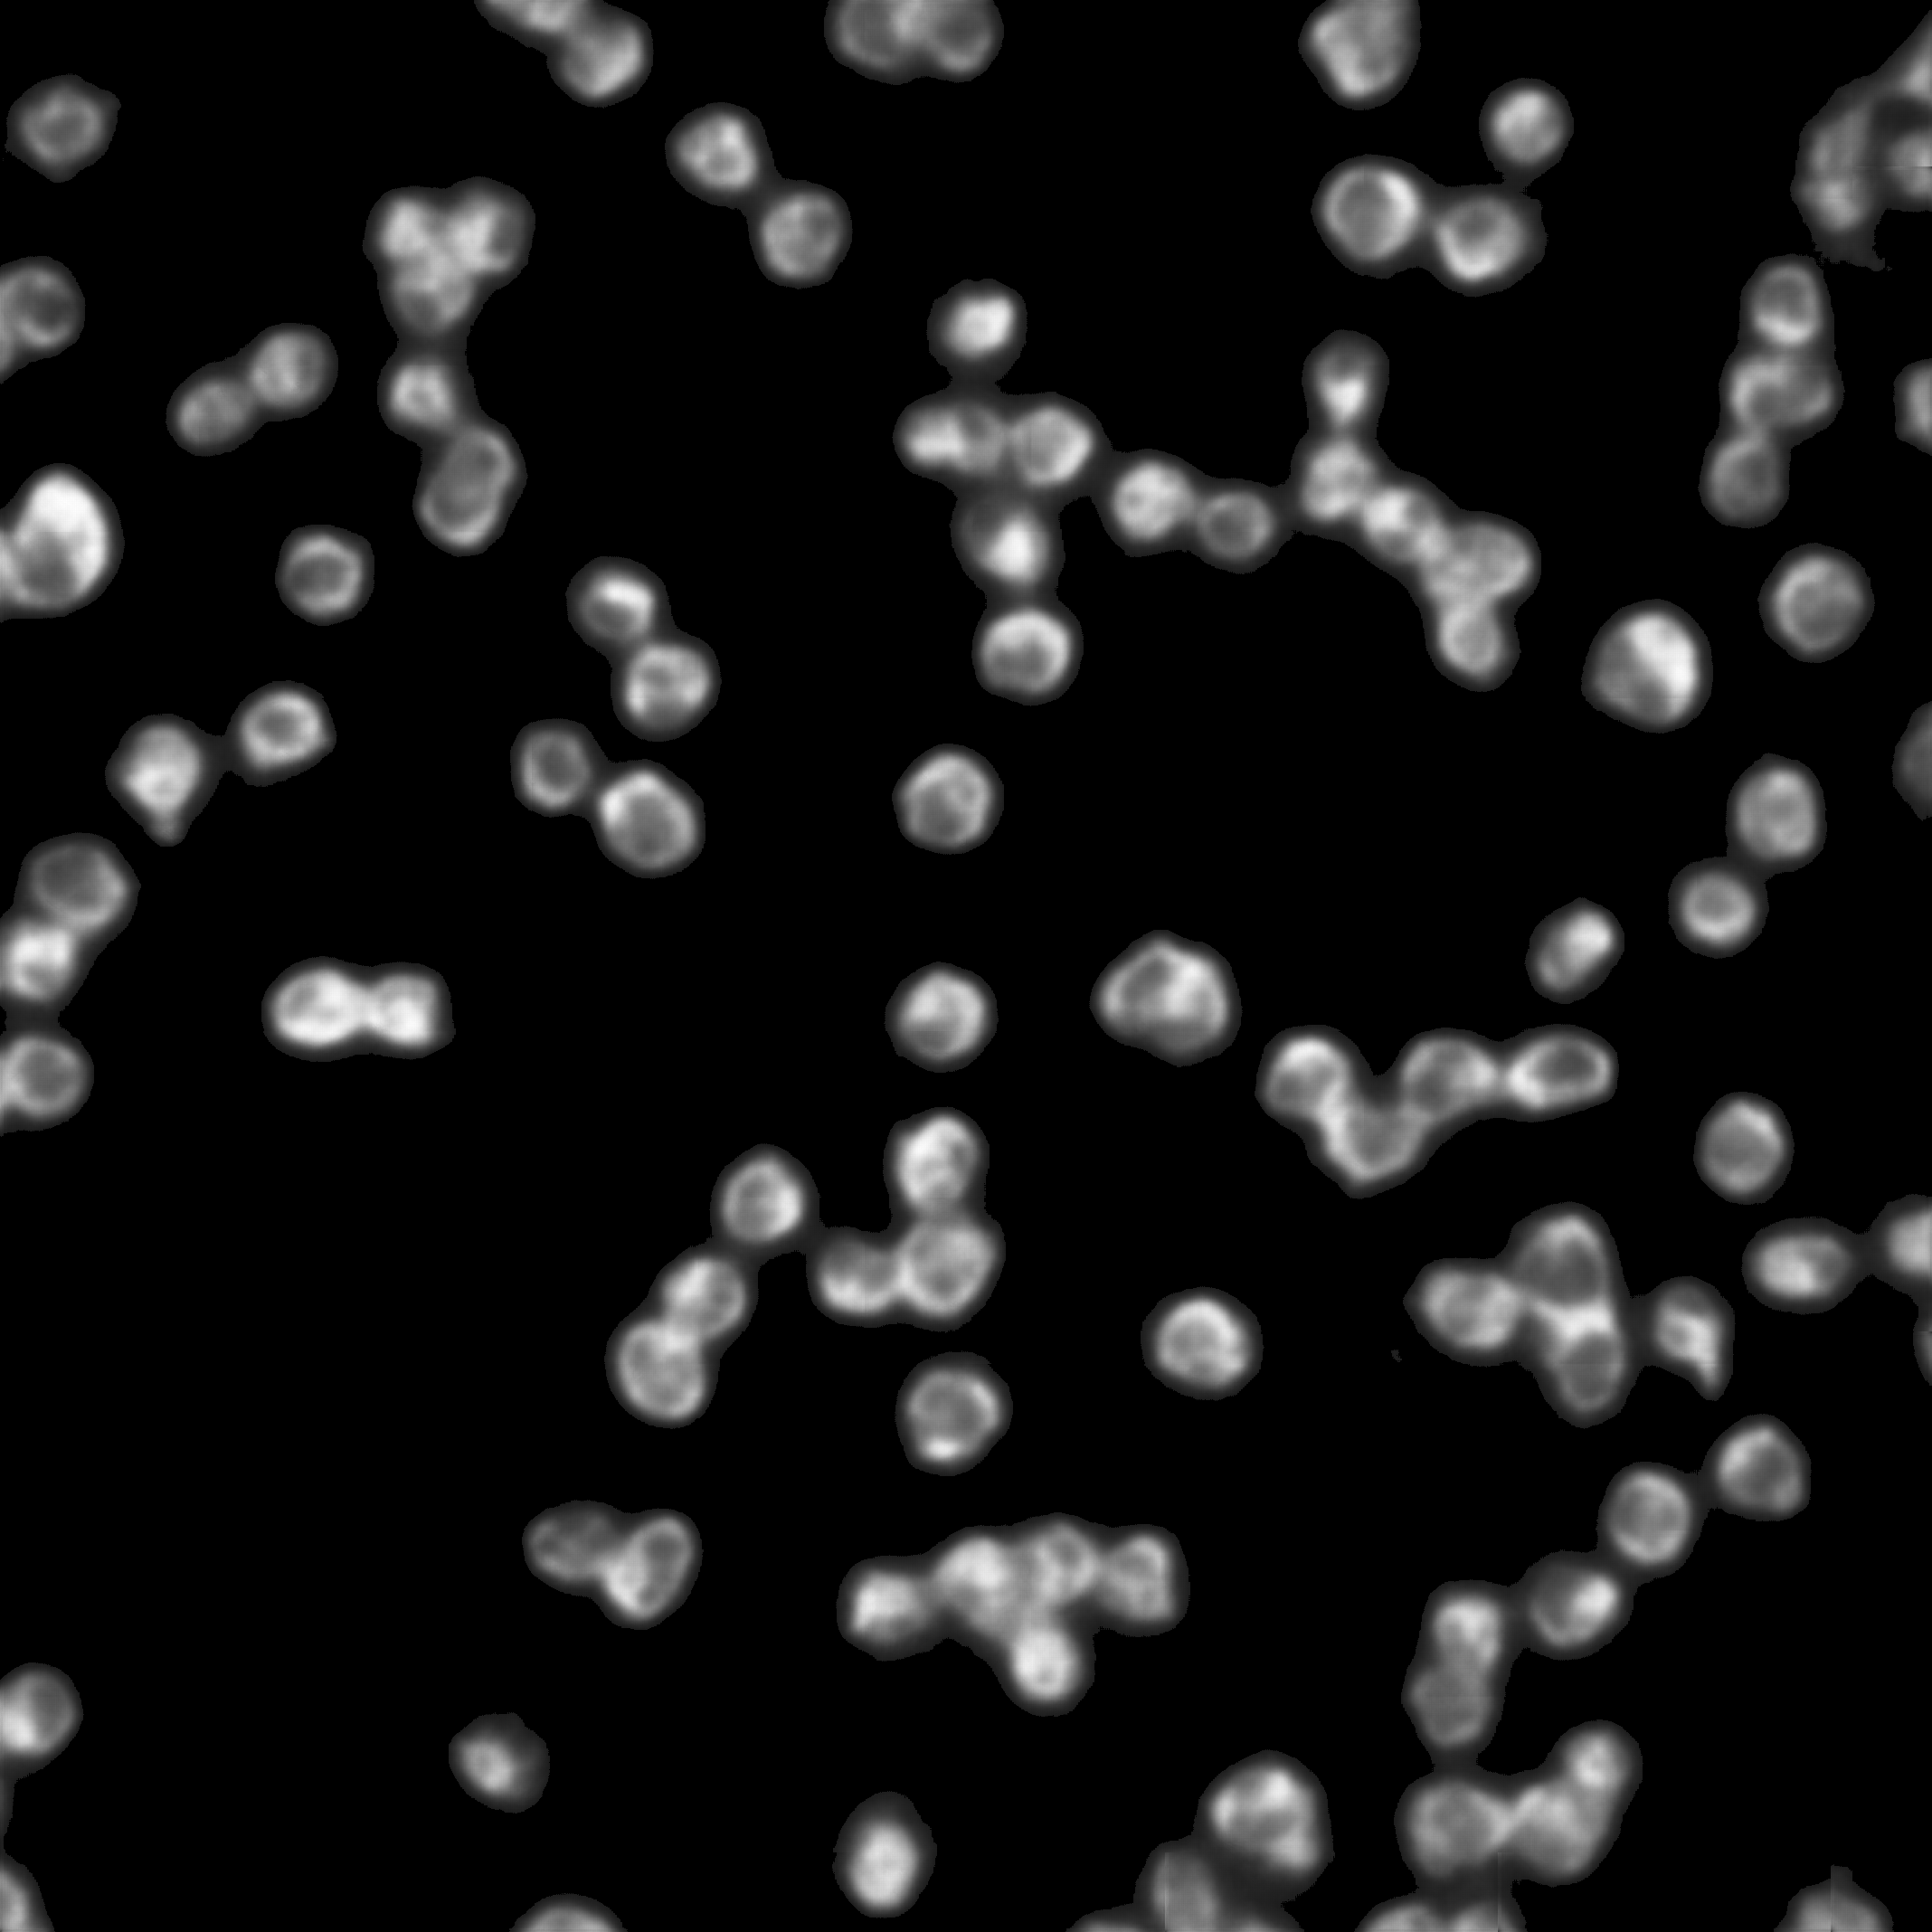
\includegraphics{bilder/ER/segmentation/pp_3.png} &
            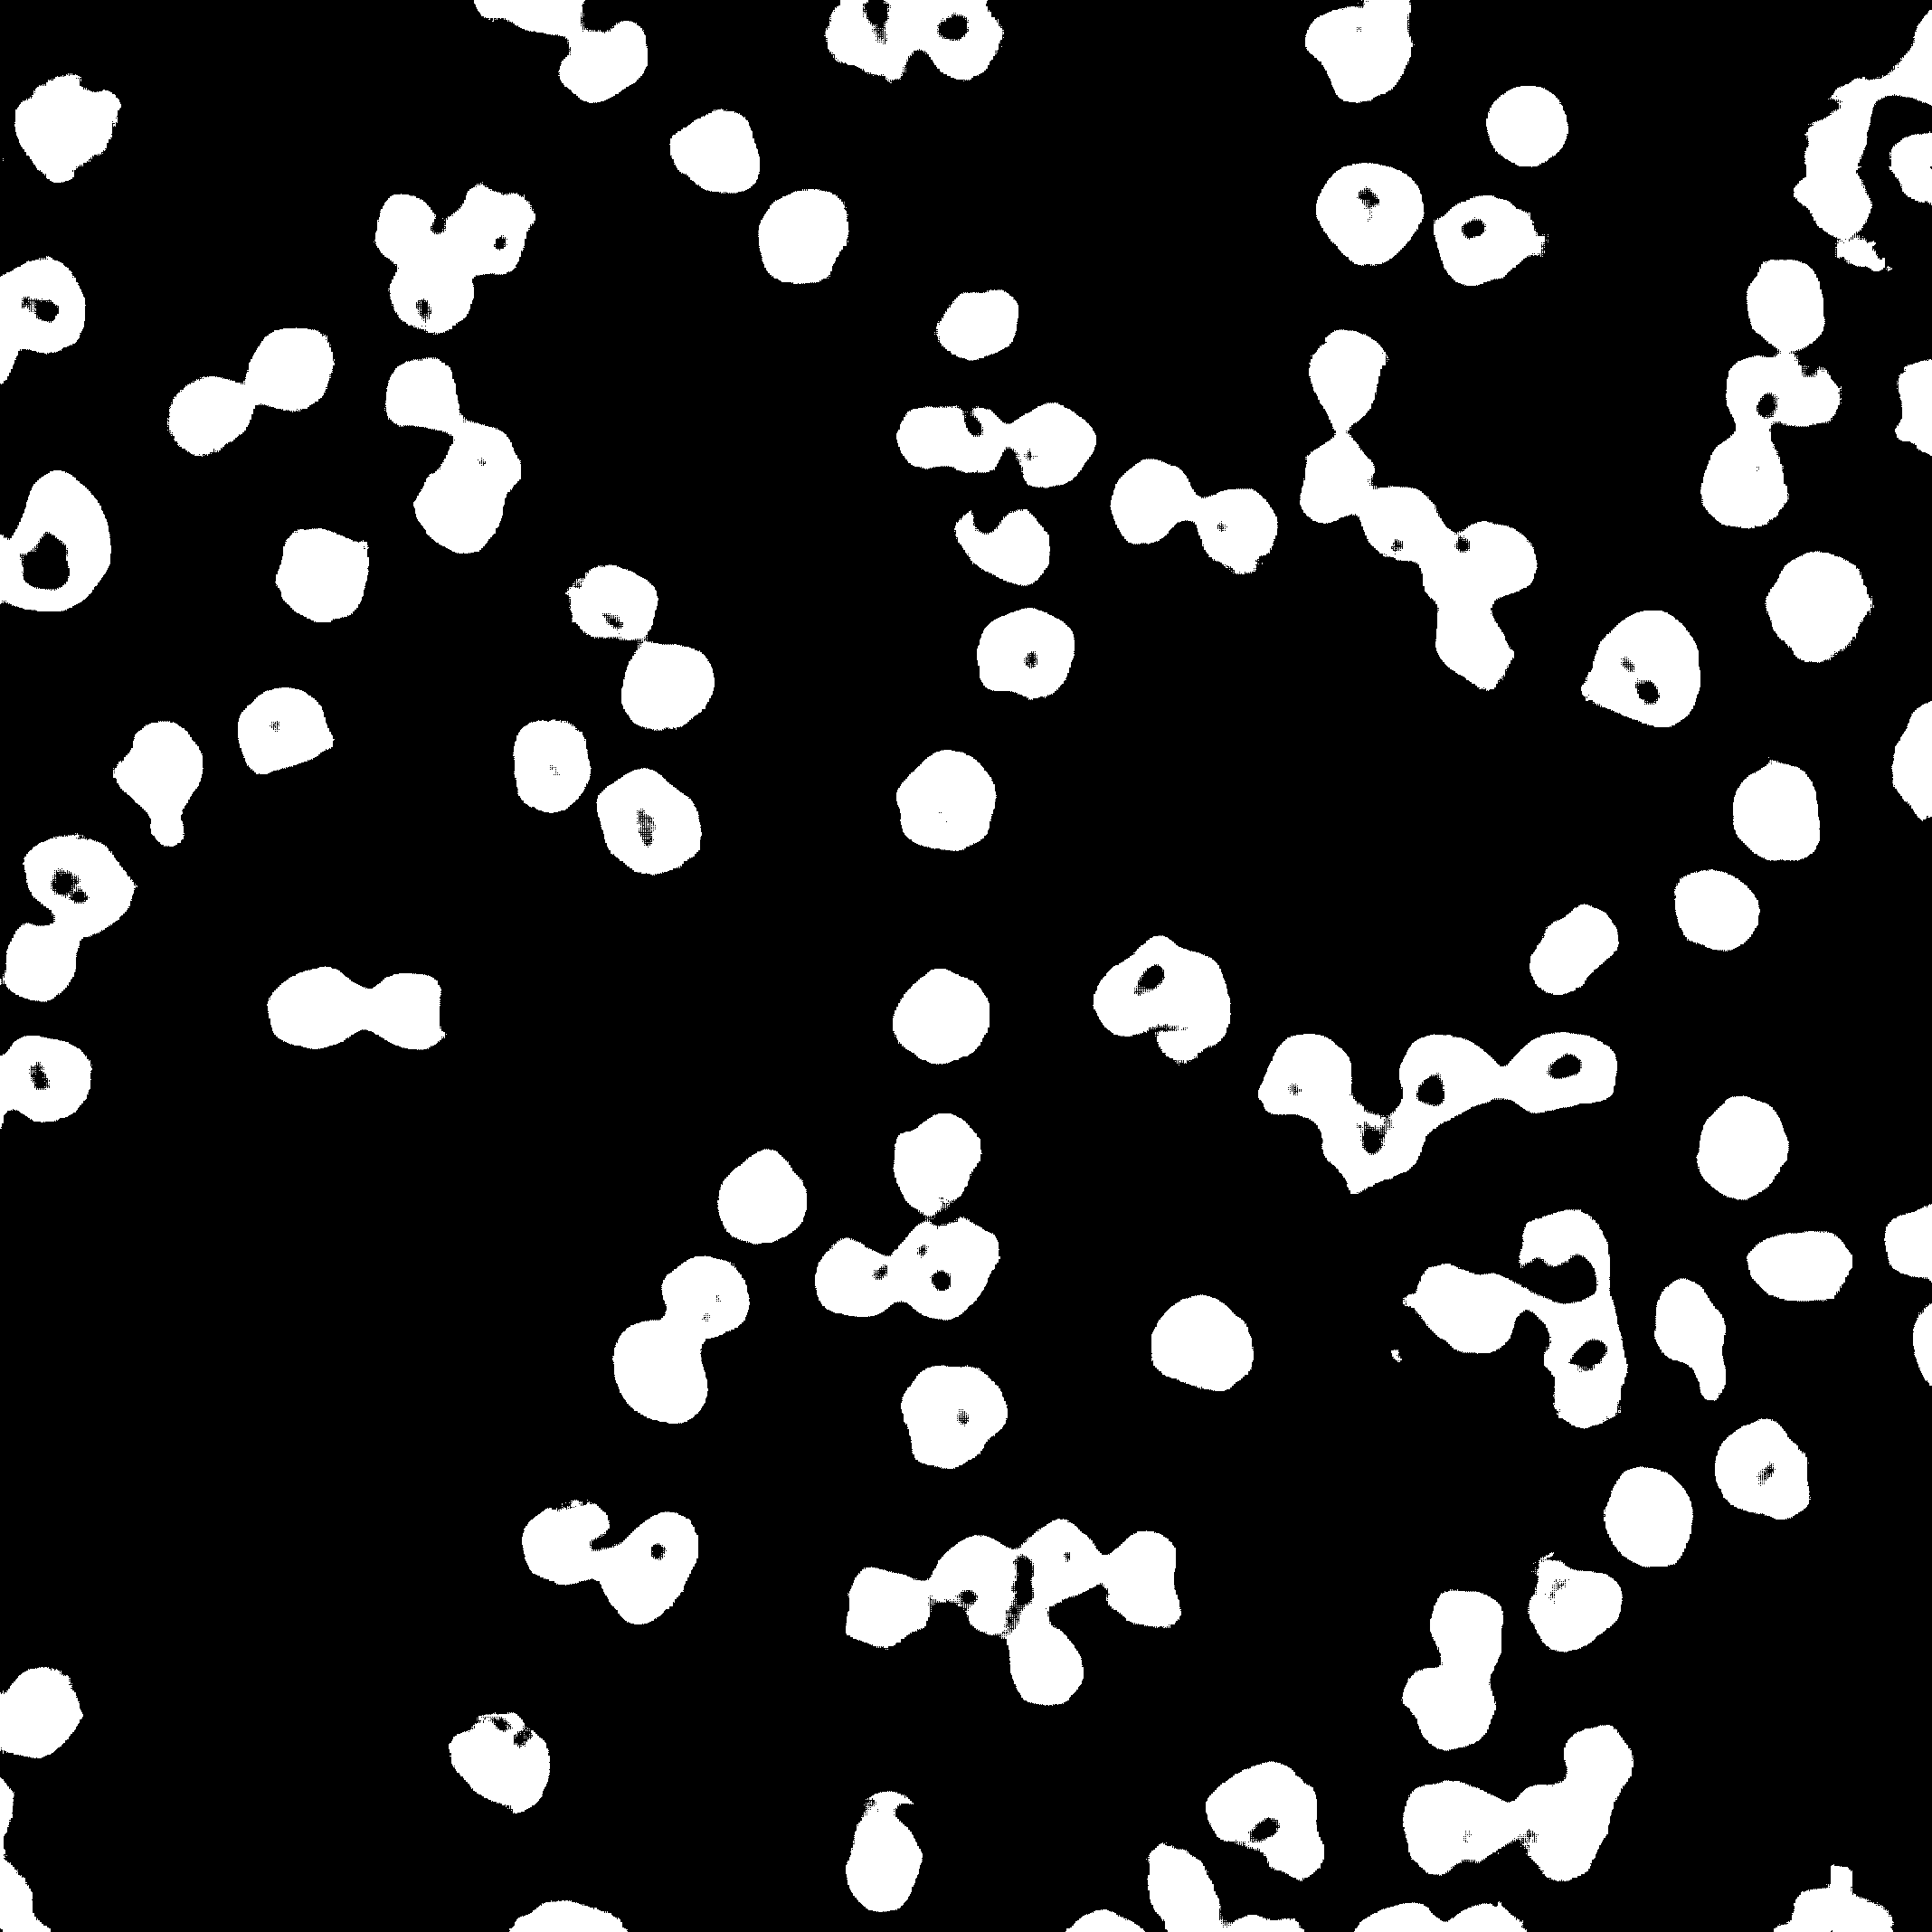
\includegraphics{bilder/ER/segmentation/pp_4.png} &
            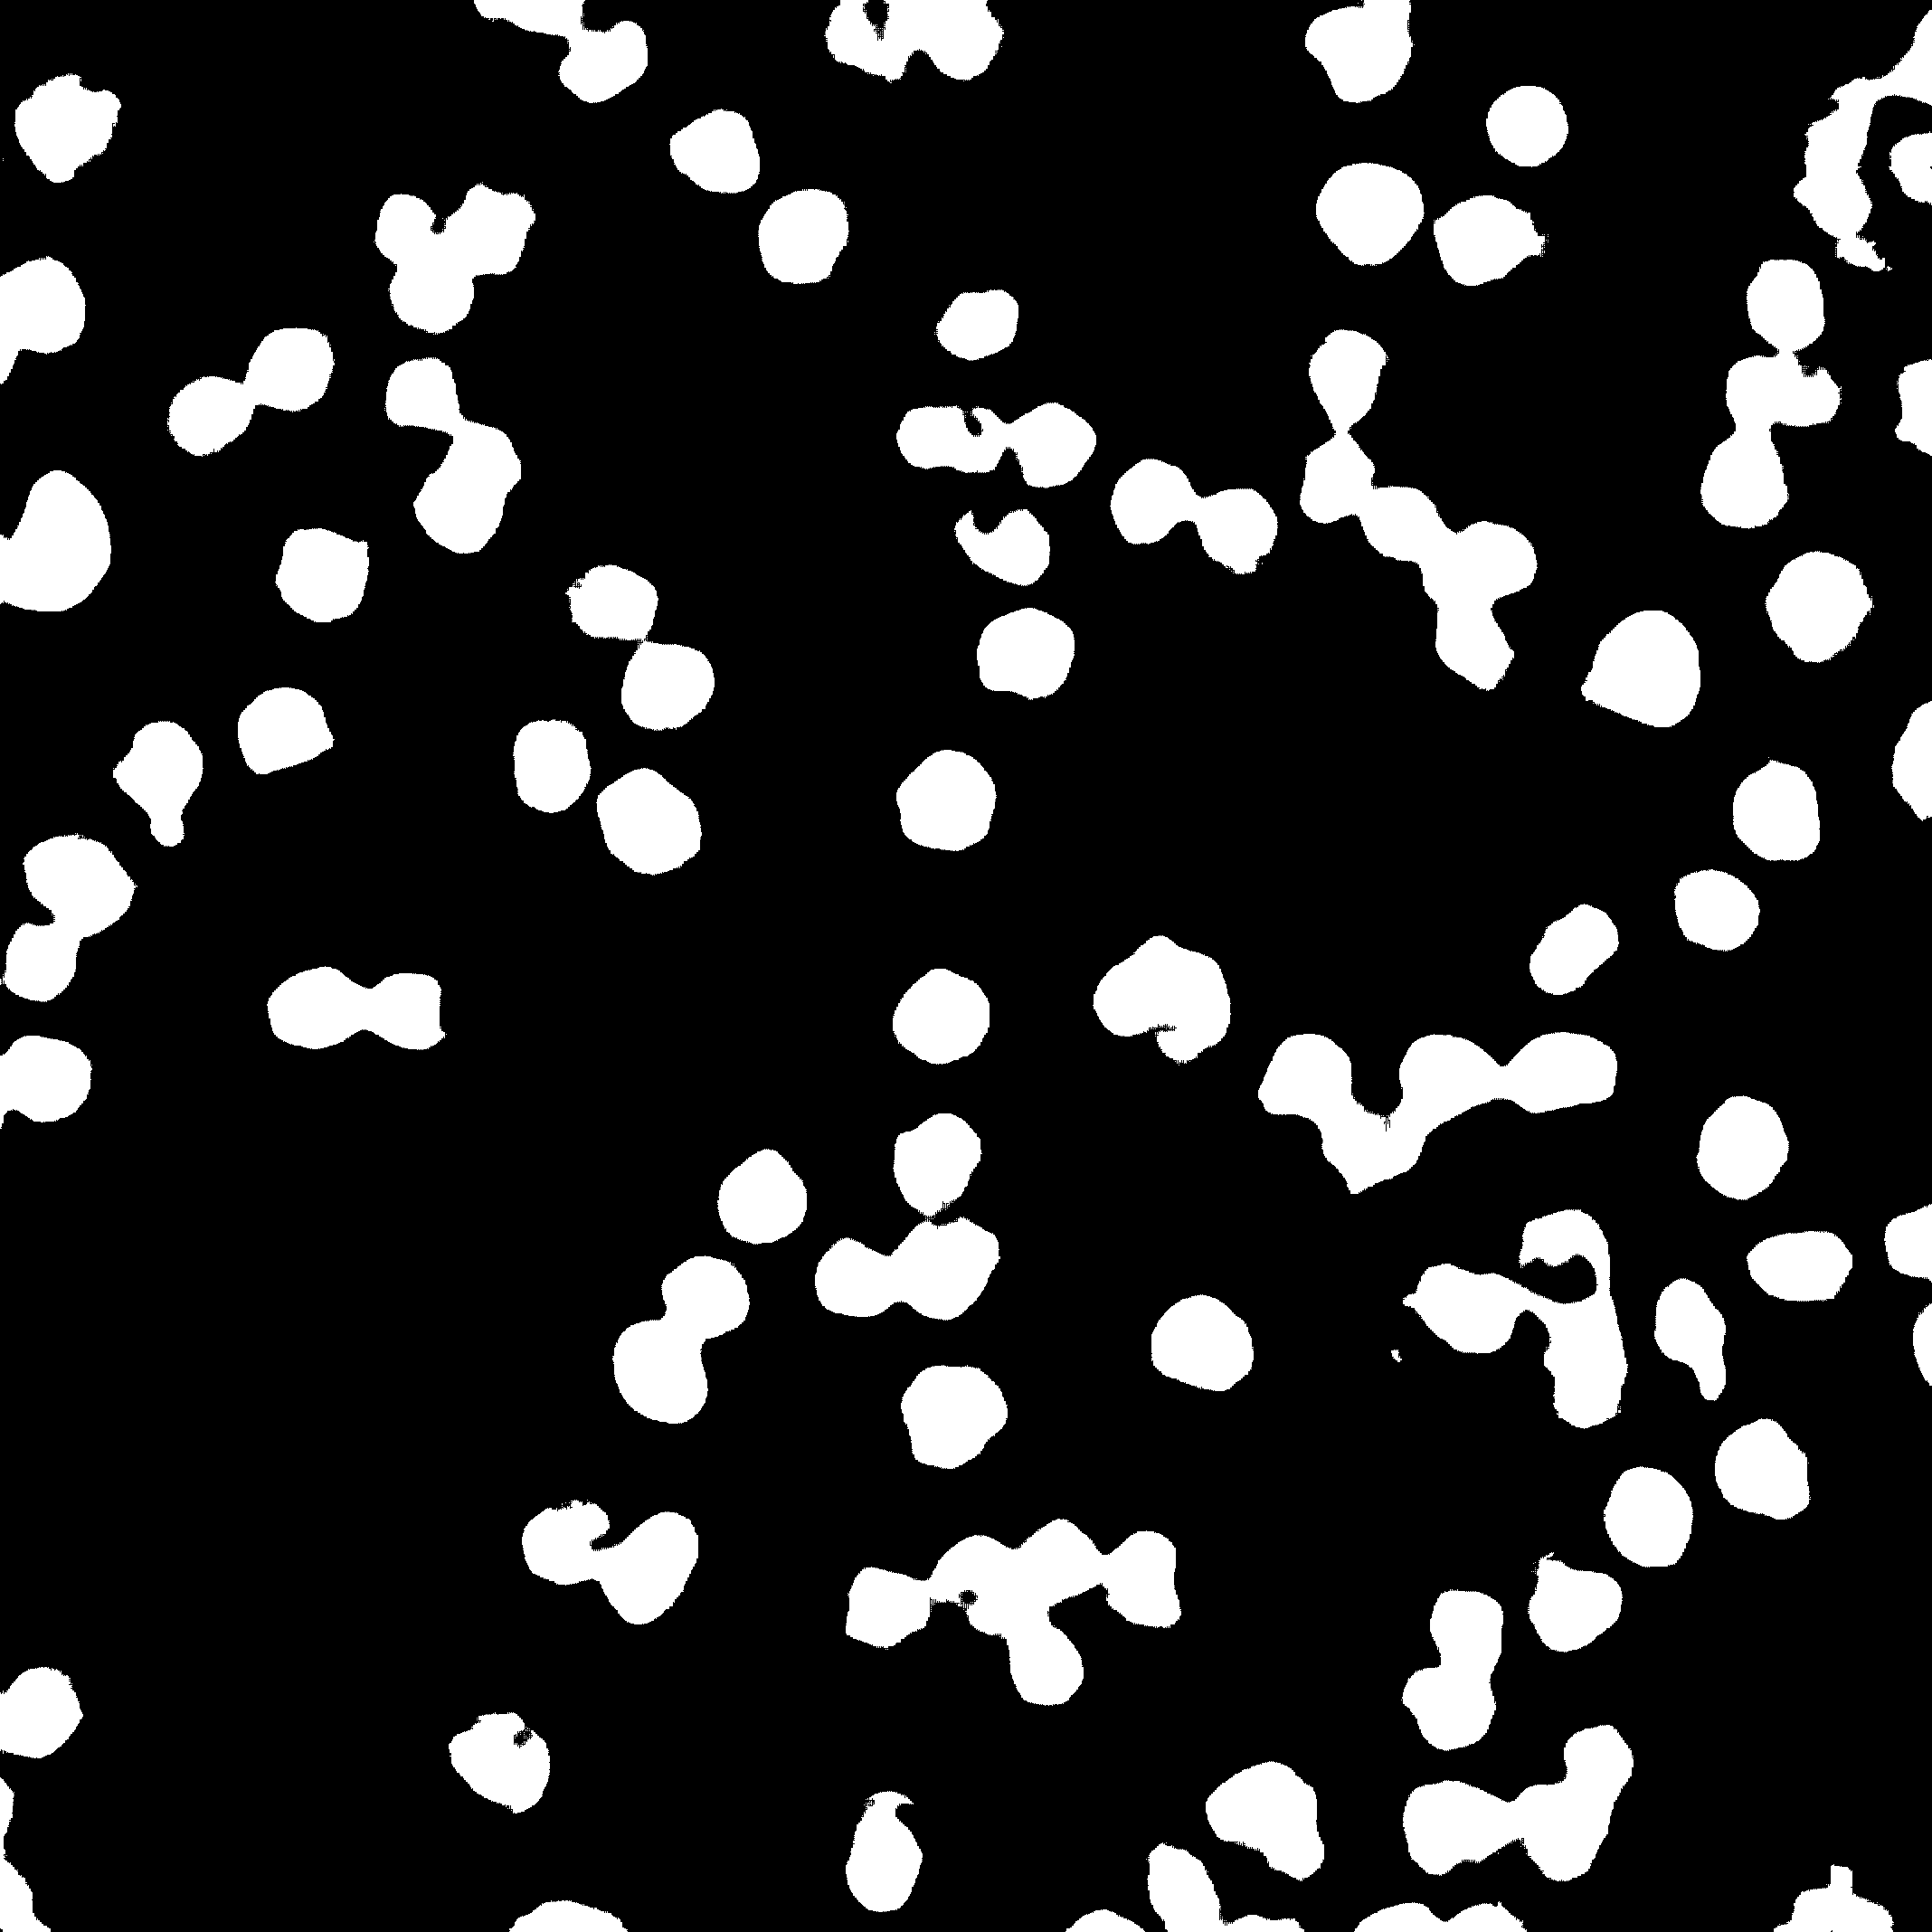
\includegraphics{bilder/ER/segmentation/pp_5.png} &
            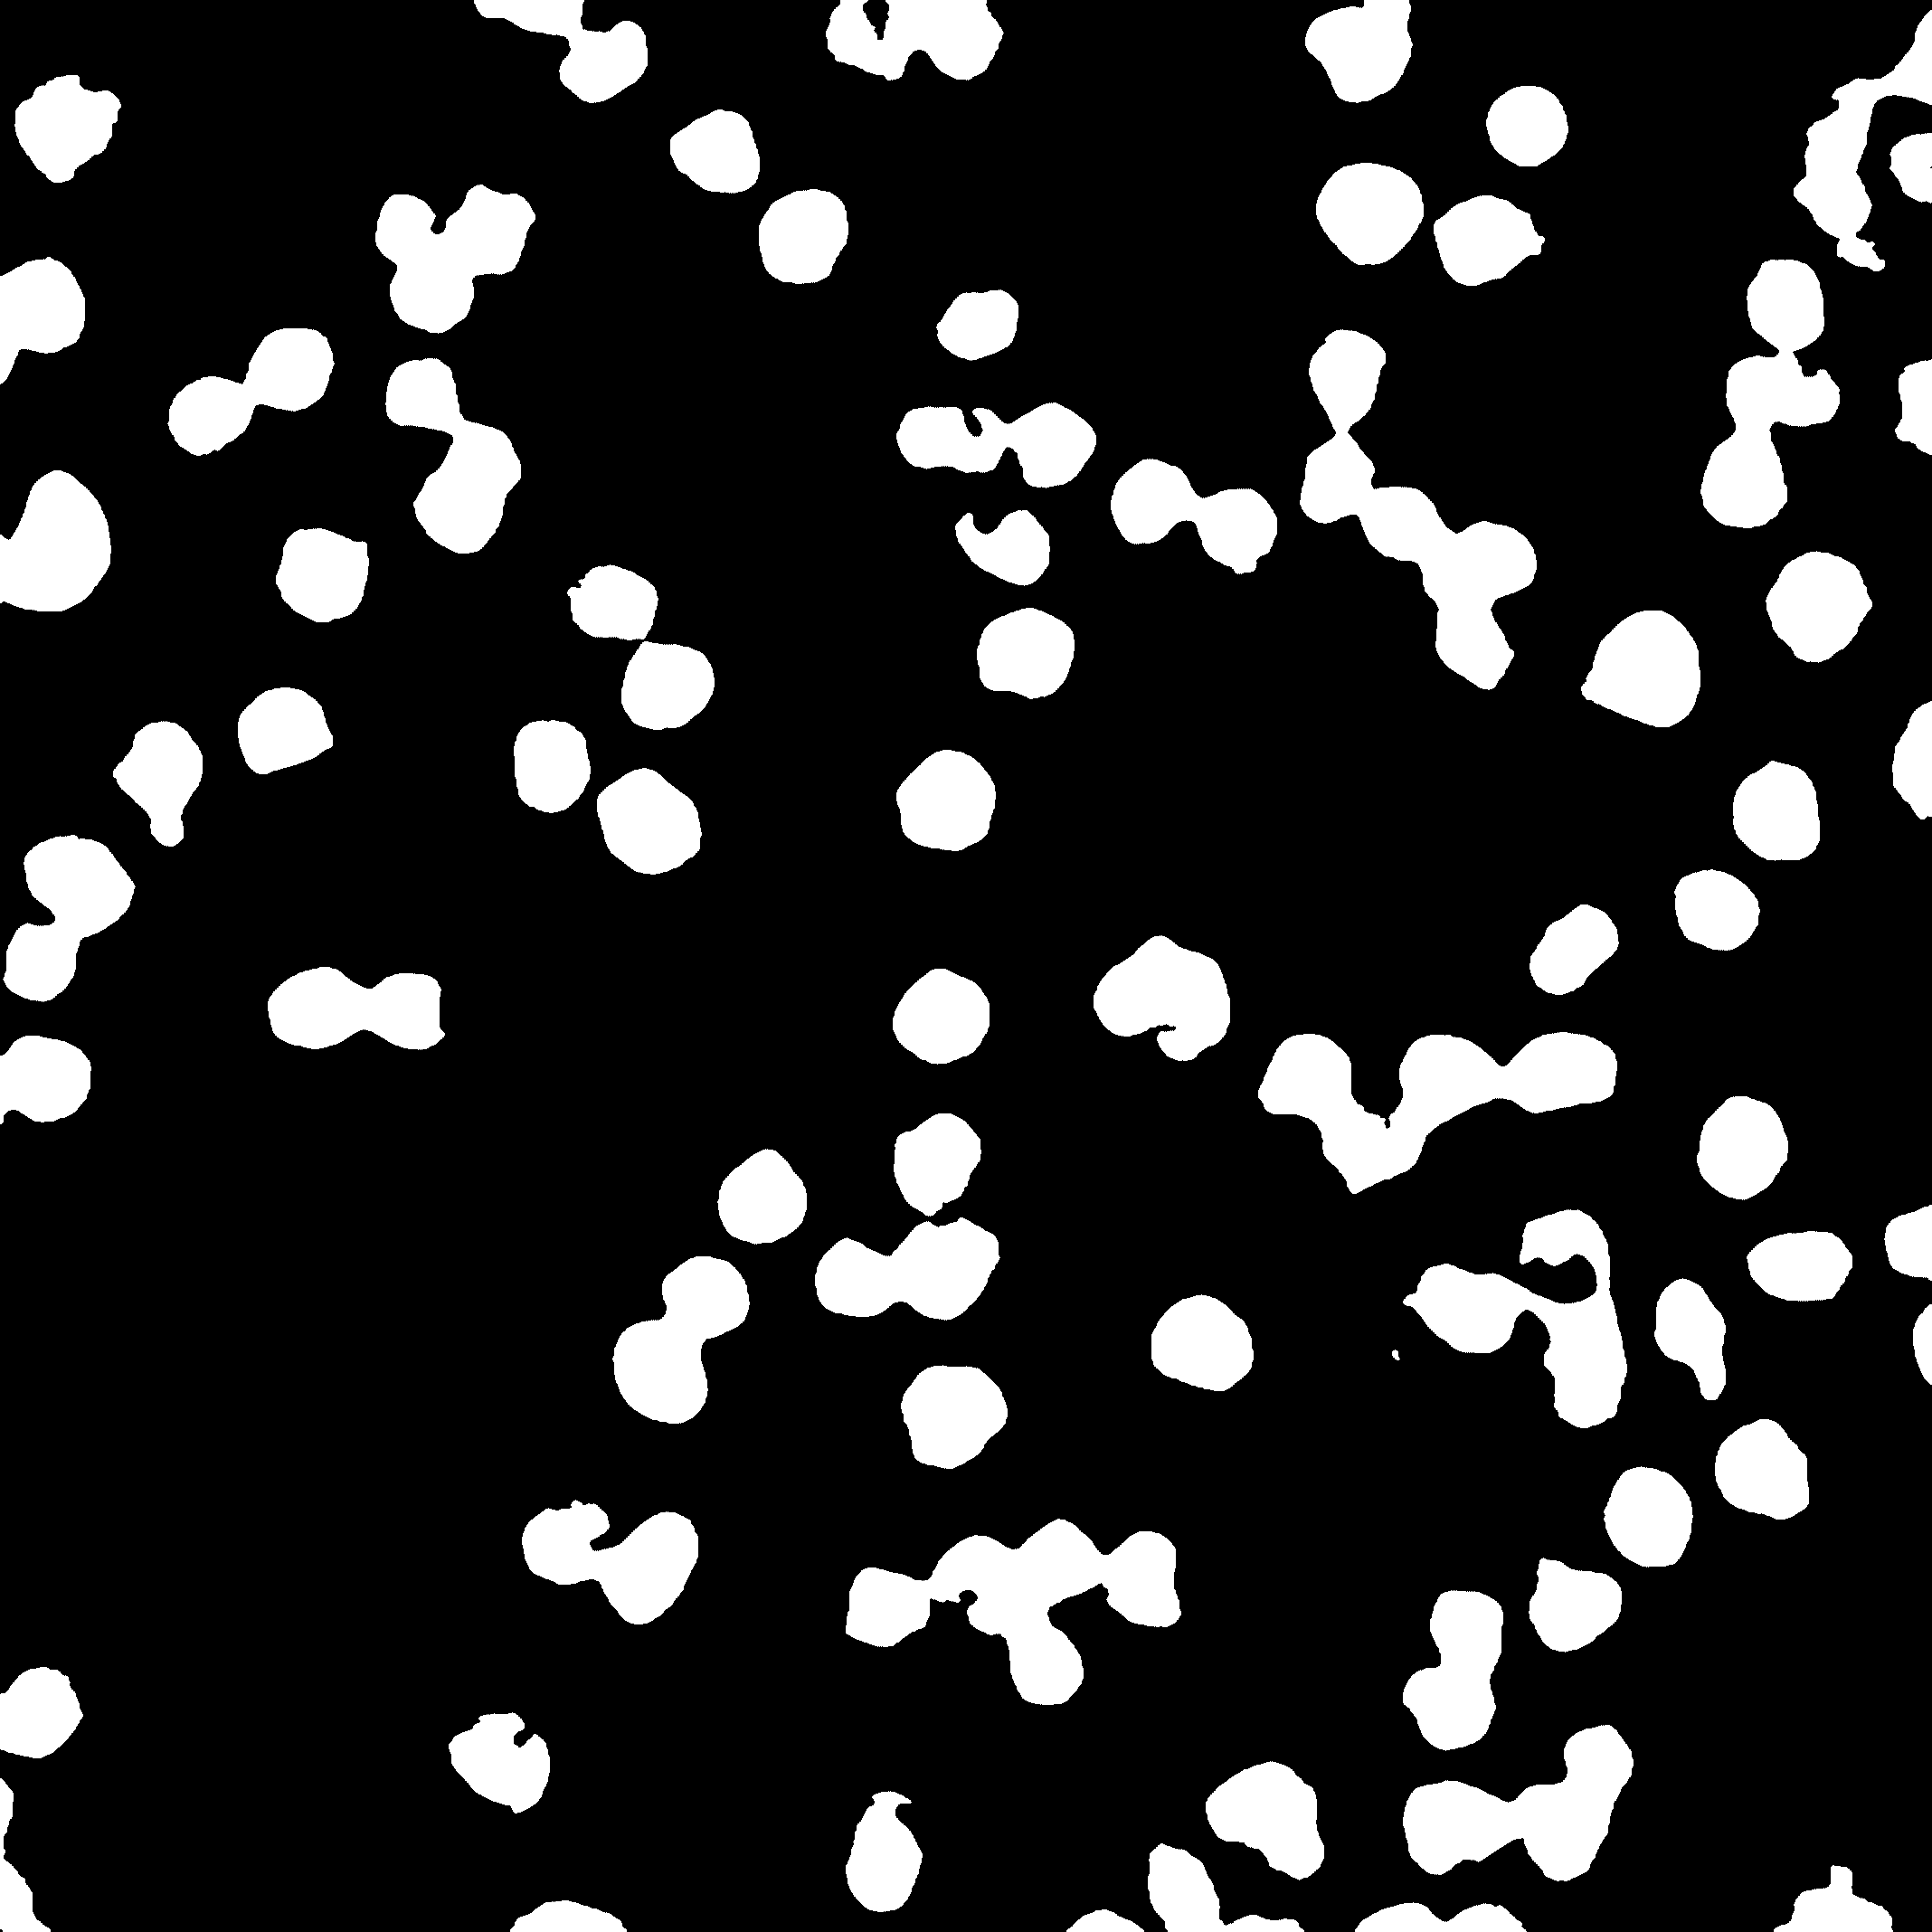
\includegraphics{bilder/ER/segmentation/pp_6.png} &
            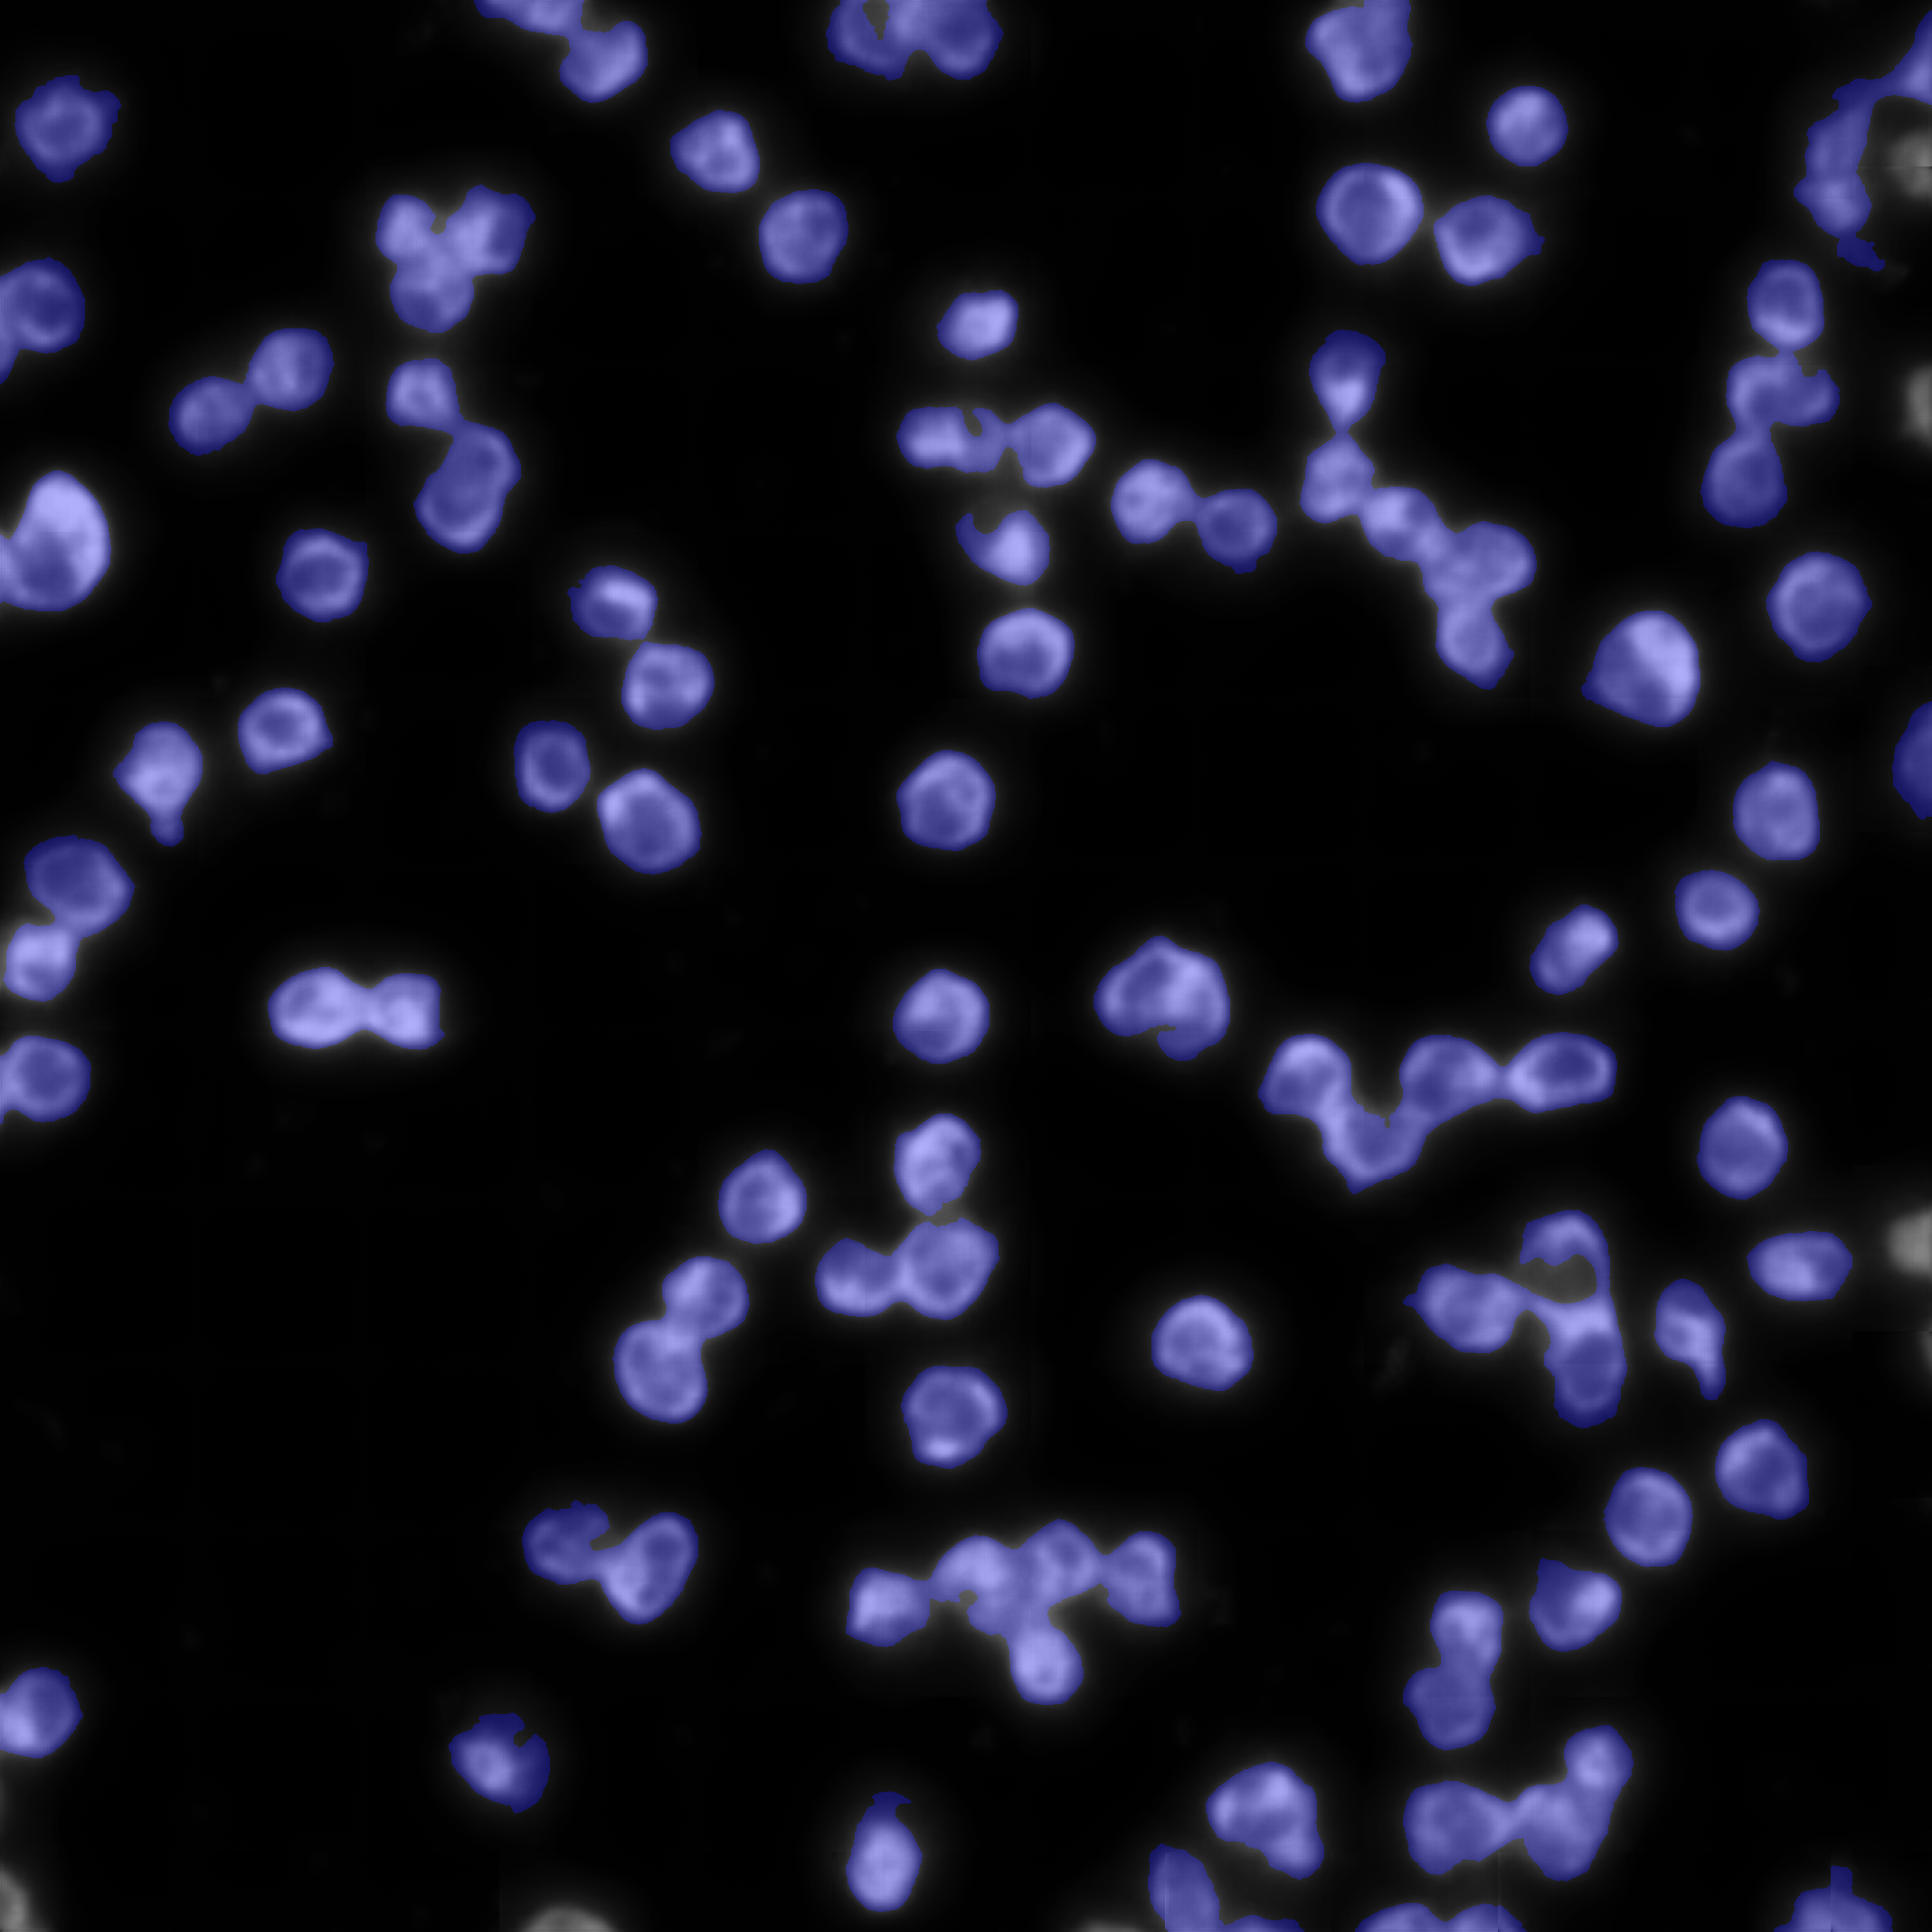
\includegraphics{bilder/ER/segmentation/pp_7.png} 
        \end{tabularx}
    \caption{ER prediction}
    \label{fig:er-prediction}
\end{figure}